\documentclass[twoside,11pt]{article}
\usepackage{amsmath}
\usepackage{graphicx}
\usepackage{subfigure}
\graphicspath{ {fig/} }
\usepackage{pdfpages}
\usepackage{csvsimple}
\usepackage{float}
\usepackage{color}
\usepackage{comment}
\newcommand\Deq{\mathrel{\stackrel{\makebox[0pt]{\mbox{\normalfont\tiny D}}}{=}}}

\newcommand{\bx}{\boldsymbol{x}}
\newcommand{\ba}{\boldsymbol{a}}
\newcommand{\bbeta}{\boldsymbol{\beta}}
\newcommand{\Gam}{\mathsf{Gam}}
\newcommand{\IGau}{\mathsf{IGau}}
\newcommand{\PG}{\mathsf{PG}}
\newcommand{\N}{\mathsf{N}}
% Any additional packages needed should be included after jmlr2e.
% Note that jmlr2e.sty includes epsfig, amssymb, natbib and graphicx,
% and defines many common macros, such as 'proof' and 'example'.
%
% It also sets the bibliographystyle to plainnat; for more information on
% natbib citation styles, see the natbib documentation, a copy of which
% is archived at http://www.jmlr.org/format/natbib.pdf

\usepackage{jmlr2e}

% Definitions of handy macros can go here

\newcommand{\dataset}{{\cal D}}
\newcommand{\fracpartial}[2]{\frac{\partial #1}{\partial  #2}}

% Heading arguments are {volume}{year}{pages}{submitted}{published}{author-full-names}

% Short headings should be running head and authors last names
\ShortHeadings{Prediction of Appointment No-shows using Electronic Health Records}{Lin, Betancourt, Goldstein and Steorts}

\begin{comment}
\ShortHeadings{Prediction of Appointment No-shows using Electronic Health Records}{\textcolor{white}{Lin, Betancourt, Goldstein and Steorts}}
\end{comment}

\firstpageno{1}

\begin{document}

\title{Prediction of Appointment No-shows using Electronic Health Records}

\begin{comment}
 \author{\name \textcolor{white}{Qiaohui Lin \email qiaohui.lin@duke.edu \\
       Department of Statistical Science \\
       Duke University\\
       Durham, NC, USA}
       \AND
       \name \textcolor{white}{Brenda Betancourt \email bb222@stat.duke.edu \\
       Department of Statistical Science \\
       Duke University\\
       Durham, NC, USA }
       \AND
       \name \textcolor{white}{Benjamin A. Goldstein \email ben.goldstein@duke.edu \\
       Department of Biostatistics and Bioinformatics\\
       Duke University\\
       Durham, NC, USA}
       \AND
       \name \textcolor{white}{Rebecca C. Steorts \email beka@stat.duke.edu \\
       Department of Statistical Science\\
       Duke University\\
       Durham, NC, USA}}
\end{comment}

%\begin{comment}
 \author{\name {Qiaohui Lin \email qiaohui.lin@duke.edu \\
       Department of Statistical Science \\
       Duke University\\
       Durham, NC, USA}
       \AND
       \name {Brenda Betancourt \email bb222@stat.duke.edu \\
       Department of Statistical Science \\
       Duke University\\
       Durham, NC, USA }
       \AND
       \name {Benjamin A. Goldstein \email ben.goldstein@duke.edu \\
       Department of Biostatistics and Bioinformatics\\
       Duke University\\
       Durham, NC, USA}
       \AND
       \name {Rebecca C. Steorts \email beka@stat.duke.edu \\
       Department of Statistical Science\\
       Duke University\\
       Durham, NC, USA}}
%\end{comment}

 
\maketitle

\begin{abstract}
Appointment no-shows have a negative impact on patient health and have caused
substantial loss in resources and revenue for health care systems. Intervention strategies to reduce no-show rates can be more effective if targeted to the subpopulations of patients with higher risk of not showing to their appointments. We use electronic health records (EHR) from a large medical center to predict no-show patients based on demographic and health care features. We apply sparse Bayesian modeling approaches based on Lasso and automatic relevance determination to predict and identify the most relevant risk factors of no-show patients at a provider level. 
\end{abstract}

\section{Introduction}

Patients that do not show to their scheduled appointment or cancel the appointment late are commonly referred in the literature as appointment \emph{no-shows}. {\color{red} A missed appointment could negatively impact patient's health condition and even increase the risk of premature death in severe cases. \cite{McQueenie19} have studied the effect of no-shows on all-cause mortality in patients with long-term mental and physical health conditions, using a 3-year period across Scotland. They have found that patients with long-term mental conditions have a higher risk of mortality if missing two or more appointments.} Other implications of no-shows range from lost revenue due to wasted resources at the moment of the appointment to future additional costs associated with the increased risk of emergency visits or hospital admissions that could have been prevented with proper follow-up during the missed appointment. For example, \cite{Kheirkhah16} reported a no-show proportion of 18.8\% across 10 clinics between the years 2006 and 2008 at a medical center that serves over 76,000 veterans in Texas, with an estimated 14.58 million marginal cost of no-shows in 2008. Other interesting studies about the costs of no-show patients and its implications in the health care system are also presented in \cite{Nuti12} and \cite{Hwang15}.

Due to the negative effects associated with missed or cancelled appointments, intervention plans to reduce the proportion of no-shows are currently a priority for health care providers and administrators. Some of the intervention practices consist of setting up reminder calls for the patients during the three days prior to the appointment, allowing immediate re-scheduling of the appointment, and reducing waiting times between the scheduling and the actual appointment dates. Recent efforts have also focused on models designed to optimize the number of overbooked patients in order to minimize loss \citep{ElSharo15}.  In this work, we are interested in prediction models that can be used to identify specific risk factors and patient subpopulations that have a higher risk of not showing to their appointments. This information can be used to aim intervention strategies to the fraction of incoming patients with highest no-show proneness. {\color{red} Notably, \cite{Williamson17} and \cite{Ellis17} have made an effort to link patients' risk of missing appointments with patient-level factors and practice-level factors in the UK.  \cite{Williamson17} used a retrospective cohort design and \cite{Ellis17} used an negative binomial model for calculating no-shows risks and a cohort analysis based on patient and practice characteristics. Our paper differs significantly from previous studies both in data structure and methodology. Our data contains summaries of previous appointments for a specific patient such as the proportion of missed appointments in the last three months and the number of times appointments were rescheduled. Using this information and other patient characteristics (demographic features, health conditions, etc) we aim to predict no-show appointments. Our study identifies possible predictors for high-risk appointment no-shows from a large sparse dataset, and we employ Bayesian statistical learning methods for this prediction task.  Here, we are able to identify the factors that significantly affect the risk of no-show appointments among hundreds of potential factors to then take specific actions such as targeted reminder phone-calls and optimal overbooking in order to reduce the risk. }

Furthermore, electronic health records (EHR) have become a powerful tool to preserve longitudinal real-time, patient-centered records that make health information available instantly. Following the work of \cite{Ben18}, we use EHR data to build a prediction model for the risk of a patient not showing to an appointment, conditional on observed individual variables that include demographic and health care features. As it is common in large health care systems, the data consists of a variety of specialties, clinics and providers serving different patient populations. \cite{Ben18} present penalized logistic models for no-show prediction across different specialties and clinics, and highlights the superior performance of clinic specific models over more general specialty level models. Here, we propose to explore models at a provider level using two approaches for penalized logistic regression within a Bayesian framework.

\begin{figure}[t]
\begin{center}
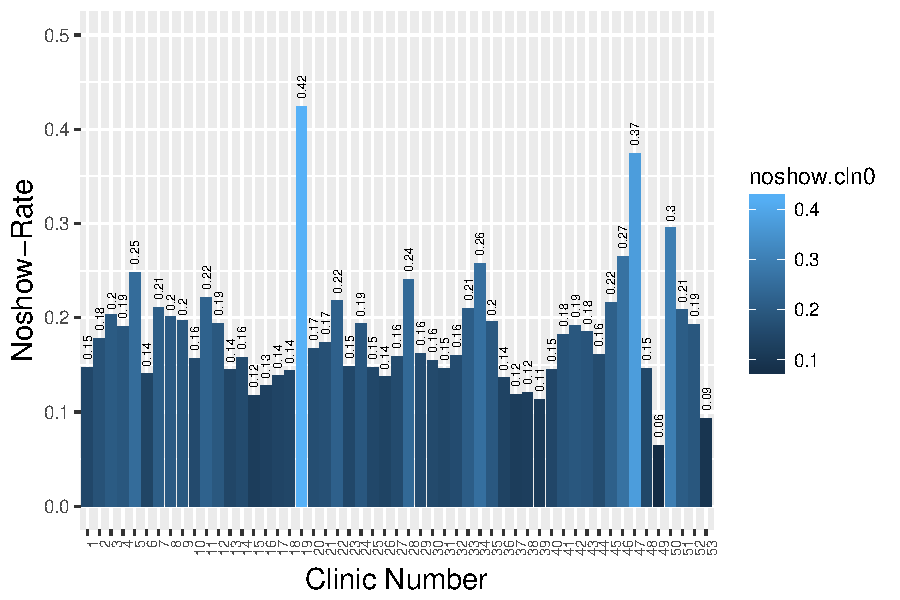
\includegraphics[width=0.7\textwidth,keepaspectratio]{fig2/eda-ns-cl-new}\\
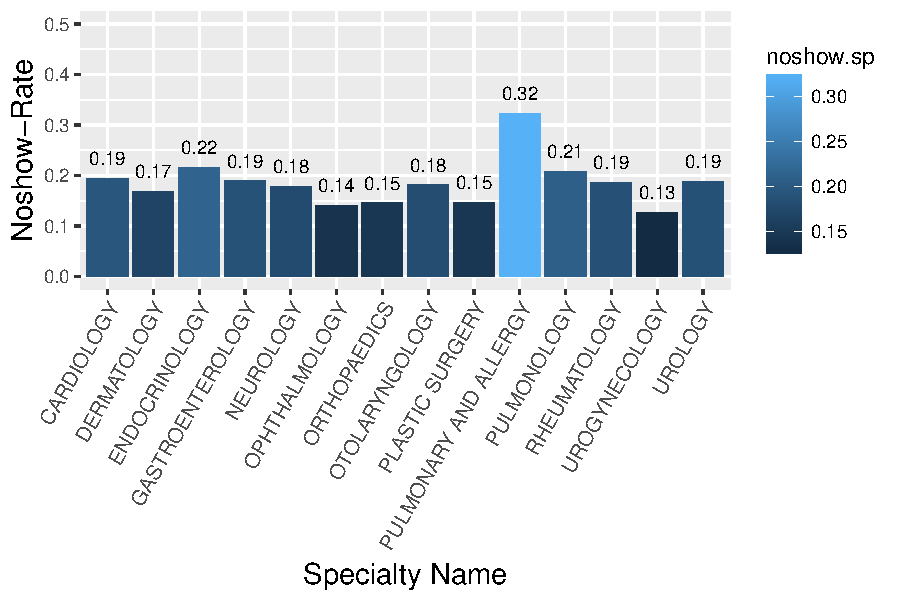
\includegraphics[width=0.7\textwidth,keepaspectratio]{fig2/eda-ns-sp}
\caption{No-show rates among different clinics (left) and specialties (right). Highest no-show rate of 42\% and lowest 6\% among clinics. Highest rate is 32\% among specialties and the lowest is 13\%. } \label{fig:Fig1}
\end{center}
\vspace{-0.8cm}
\end{figure} 

 
\section{EHR Data}

Electronic health records collected from a large academic medical center in North Carolina consists of over 2 million patients between the ages of 18 and 89 years of age who had an appointment at an outpatient specialty clinic between 2014 and 2016. A total of 14 specialties (Cardiology, Neurology, Gastroenterology, Ophthalmology, Dermatology, Endocrinology, Orthopedics, Otolaryngology, Plastic Surgery, Pulmonary and Allergy, Rheumatology, Urogynecology and Urology) are included in the data. Many specialties have multiple clinics serving different volumes of patients from distinct populations (age, gender), for a total of 61 clinics that can be either attached to or detached from the primary hospital. For the purpose of this analysis we removed 8 small clinics that did not have enough data to train the models for a total of 53 clinics and 475 providers. 

Patients were required to have made the appointment at least three days before the appointment date, and received call reminders via an automated phone system. The definition of ``late cancellation" differed among clinics depending on rescheduling difficulty. In this application, we defined a late cancellation as cancelling on the day of the appointment. Appointments that were canceled prior to one day were not considered as no-shows in this analysis. The outcome of interest is then an observed binary variable representing whether a patient did not show to their scheduled appointment or canceled on the day of the appointment. In this particular EHR dataset, the average no-show rate across specialties is approximately 18\%. Figure \ref{fig:Fig1} displays how the no-show rate varies across different clinics and specialties. The highest no-show rate among clinics is 42\% for a clinic in the Pulmonary and Allergy specialty and the lowest is 6\% for a clinic in Orthopedics. The highest no-show rate among specialties is also present in the Pulmonary and Allergy specialty (32\%), and the lowest rate in the Urogynecology specialty (13\%). 

\begin{figure}[h]
\begin{center}
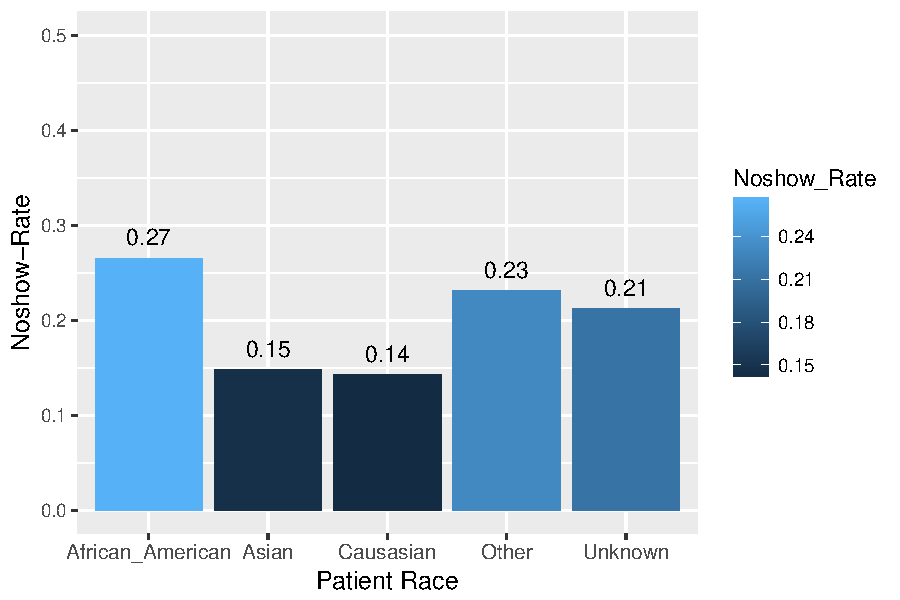
\includegraphics[width=0.47\textwidth]{fig2/eda-ns-fta}
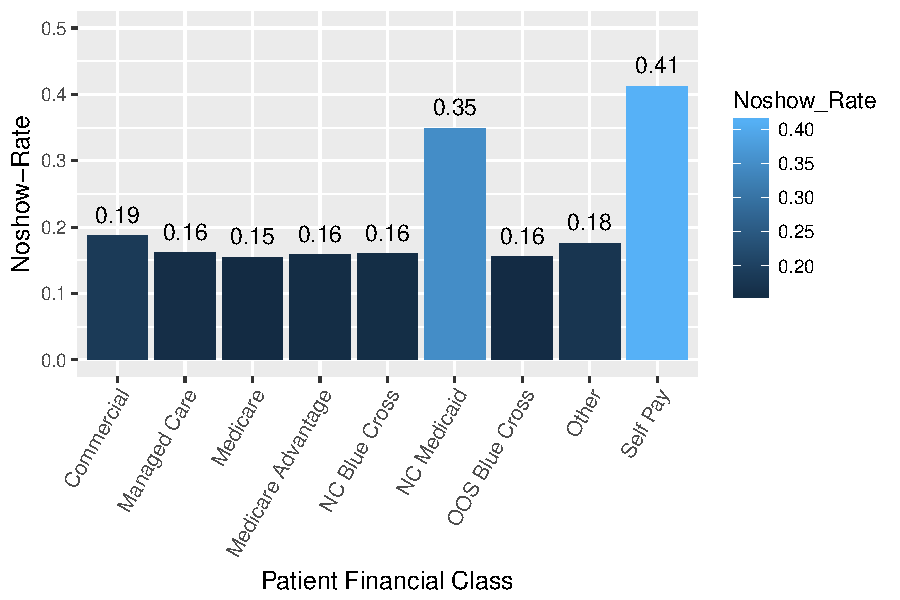
\includegraphics[width=0.47\textwidth]{fig2/eda-ns-ftb}
\caption{No-show rates by patient race and financial class. African American patients and patients in the Self Pay category have higher no-show rates.}\label{fig:Fig2}
\end{center}
\vspace{-0.5cm}
\end{figure}

The data also contains information about representative patients demographics (age, gender, employment status), health care plan, engagement with the health system (active in the online patient portal MyChart, response to 7 day phone call), appointment type (how long the appointment was held for, the location of the appointment), patient response to appointment confirmation among others, for a total of 67 covariates (102 when using dummy variables for categorical features). There is little clinical information available except for substance abuse and psychiatric diagnosis in the past two years. The available patient information is utilized to model the no-show probability of individual patients and to identify high-risk patients for which intervention measures can be directed in order to reduce no-shows rates. 

Figure \ref{fig:Fig2} displays the no-show rates among groups for two features: race (demographic information) and medical financial class (health care information). We observe that the highest no-show rates are present among African American patients, and in the self-pay category of financial class that corresponds to uninsured patients that are usually responsible for full payment of the medical care they receive. We want to point out here that in scenarios where predictive policing is of interest it is of utmost importance to avoid perpetuating discriminatory practices against certain subpopulations. In this particular application, attributes such as race and socio-economic status may be predictive of no-shows, but implementation of preventive measures based on these attributes should be carried out with care. For example, direct application of the finding that African Americans are less likely to show up for their appointments, could lead to discriminatory practices like overbooking appointments for all African American patients. The ethical implications of automated machine learning approaches and other relevant issues associated with causality and fairness are discussed in depth in \cite{Kusner17}.

In this particular data set, and possibly in other EHR data sets coming from large medical institutions, there is a natural specialty-clinic-provider hierarchy. The 53 clinics considered in this data are served  by 475 individual medical providers (doctors) that handle between 1,005 and 21,560 patients each, with and average of 4,404 patients overall. The provider with the largest number of patients is observed in the ophthalmology specialty, and a few providers serve in more than one clinic at a time. We see that the average no-show rate among providers varies widely between 1.6\% and 97\% with an average rate of 17\%. In this work, we choose to build separate risk models at a provider level to take into account the possible heterogeneity among the population of patients. The multiple risk models would also allow us to perform a more exhaustive identification of the different underlying risk factors of no-shows by provider considering that they differ among clinics and specialty combinations \citep{Ben18}. 

\section{Methods}

We employ a logistic regression model for each provider where the response is the binary variable indicating whether a patient is a no-show or not, and the predictor variables are all the demographic and health care attributes available in the EHR data. This model choice allows us to predict the probability of a patient being a no-show, and estimate the change in risk associated with a particular factor level or value increase of a predictor variable.

Let $y_{i}$ denote the no-show status of the i-th patient for a specific provider. The proposed model assumes independent Bernoulli distributions on the outcome $y_i$ as follows:
\begin{align}
y_{i} & \stackrel{iid}{\sim} Bernoulli (p_{i}) \quad i=1,\ldots,n
\end{align}
where $p_{i}$ is the probability for patient $i$ of being a no-show:
\begin{equation}
p_{i} = P(y_i=1|\bx_i,\bbeta)=\frac{1}{1 + exp(-\bx_i\bbeta)},
\end{equation}
for $\bx_{i}$ a $p$-dimensional vector of individual attributes, and $\bbeta$ the respective vector of regression coefficients associated with $\bx_{i}$. Hence, the likelihood function is given by, 
\begin{eqnarray} \label{eq:lik}
f(X;\bbeta) = \prod_{i=1}^n\frac{\exp(x_i\bbeta)^{y_i}}{1+\exp(x_i\bbeta)}.
\end{eqnarray}

In a relatively high-dimensional application like the one presented here, it is important to consider the issue of variable selection in the model. The number of features present in the EHR data is relatively large ($p=102$) and we are interested in identifying the relevant risk factors of no-shows among providers. While building separate models is straightforward, performing variable selection among a large number of models can be challenging. Here, we rely on sparse Bayesian approaches to identify the more meaningful no-show predictors by provider in an automatic fashion. In the following section we discuss two well known machine learning methods for sparse learning that also belong in the class of
hierarchical shrinkage priors for regression models.   

\subsection{Lasso Penalized Logistic Regression}

Among the most popular approaches for variable selection in regression models are those based on Lasso (least absolute shrinkage and selection operator) introduced by \cite{Tibshirani96}. In Lasso regression, a  penalty is imposed on the model coefficients to induce sparsity such that the less relevant variable coefficients are shrunk to zero, thus performing automatic variable selection. Furthermore, prediction accuracy can also be improved by shrinking the model coefficients. More specifically, the estimates for the model parameters in traditional Lasso are obtained by solving:
\begin{equation} \label{eq:lasso}
\max_{\bbeta}  \mathcal{L}(\bbeta) - \lambda \sum_{j=1}^p|\beta_j|
\end{equation}
where $ \mathcal{L}(\bbeta)$ is the log-likehood based on equation (\ref{eq:lik}) and the second term corresponds to the Lasso penalty. The parameter $\lambda > 0$ is the penalty parameter that controls the shrinkage level of the coefficients towards zero, and therefore has a direct impact on the quality of the estimates and predictions generated by the model. 

The penalty parameter $\lambda$ can be selected through cross-validation by training the model on a fraction of the observed data (training set) for each provider, and performing predictions on the remaining portion (testing set) for a grid of values of $\lambda$. For evaluation of prediction performance, these predictions can be compared against the respective observed no-show indicator, then the number of false and true positives is computed, and a receiver operating characteristic (ROC) curve is constructed. Finally, the optimal penalty parameter can be chosen as the value of $\lambda$ in the grid that provides the highest area under the curve (AUC) in the testing dataset. The main drawback is that selection of the optimal tuning parameter through cross-validation can be computationally expensive in general \citep{Tibshi05}, and in particular in this application where we fit independent models for each provider and the range of values of $\lambda$ can vary among them. 

Here, we adopt the Bayesian counterpart of Lasso regression presented in \cite{ParkCasella08} where the penalty parameter can be estimated directly by assuming a prior distribution on $\lambda$. The Bayesian Lasso was introduced by noting that the Lasso penalty in equation (\ref{eq:lasso}) is equivalent to assuming independent Laplace prior distributions on the regression coefficients. \cite{ParkCasella08} provide a hierarchical model and Gibbs sampler in the linear regression context by representing the Laplace distribution as a scale mixture of normals. In particular, a conditionally conjugate Gamma prior $\lambda^2 \sim \Gam(r,\delta)$ is assumed for the penalty parameter, and thus posterior samples of $\lambda$ can be obtained in a straightforward fashion from a Gamma distribution with updated parameters. This is a very appealing feature for this application but a full Bayesian approach also comes with its own set of limitations. The main disadvantage is that inferences obtained through a Bayesian framework lack direct variable selection. While the traditional maximum a posteriori approach in equation (\ref{eq:lasso}) produces estimates of the coefficients that are exactly zero, the Bayesian counterpart of \cite{ParkCasella08} does not. However, variable selection in this setting can be guided by using the credibility intervals of the model coefficients. We discuss in more detail how to identify relevant risks predictors using credibility intervals in the context of the no-shows application in Section \ref{sec:application}.

In order to perform Bayesian inference with a binomial likelihood, we exploit the data augmentation
method based on Polya-Gamma latent variables proposed by \cite{PolsonScott13}. Using this approach, the binomial likelihood can be represented as a mixture of
normals with Polya-Gamma mixing distribution. This approach allows for a full conjugate
hierarchical representation of the Bayesian lasso model and posterior inference through relatively simple Markov chain Monte Carlo (MCMC) algorithms. Specific theoretical guarantees for Gibbs sampling of Bayesian logistic regression with Polya-Gamma latent variables are provided in \cite{ChoiHobert13}. Details of the full conditional distributions of the Gibbs sampling algorithm for the Lasso penalized logistic regression setting are presented in Appendix A.

\subsection{Logistic Regression with Automatic Relevance Determination}

Even though the Bayesian Lasso has been widely used in many applications, there are other common alternatives for prior distributions that induce sparsity on model parameters. For example, the sparse Bayesian learning approach for regression introduced by \cite{Tipping00, Tipping01} is considered a type of automatic relevance determination (ARD) that is also an effective tool for trimming large numbers of irrelevant features by inducing sparse solutions. Bayesian Lasso and ARD both accomplish variable selection in a linear regression setting by assigning a shrinkage prior on coefficients where posteriors for irrelevant variables would converge to zero. The key difference lies in the choice of the prior distribution for the regression coefficients. Instead of assigning a Laplace prior as in the Lasso case, the prior used for the implementation of ARD is a member of the scale mixtures of normals and therefore inherits its appealing conjugacy properties. 

In particular, independent  Normal prior distributions are assigned to each $\beta$,
\begin{equation}
P(\bbeta|\ba)= \prod_{j=1}^{p} \N(\beta_{j}| 0, a^{-1}_{j}),
\end{equation}
where $\ba=(a_1, a_2, \ldots, a_p)$ is a hyperparameter vector of precisions that controls how far from zero the coefficients can be. The precision hyperparameters are assigned Gamma prior distributions, 
\begin{equation}
P(\ba)=\prod_{j=1}^{p} \Gam(a_j|a_0,b_0),
\end{equation}
where $a_0$ and $b_0$ represent the shape and rate parameters, respectively. This hierarchical prior specification simply leads to Normal-Inverse Gamma prior distributions for each regression coefficient. Here, low precision means the prior is uninformative while high precision means $\beta_j$ is constrained to be zero, and thus the corresponding feature is very likely irrelevant. This prior choice will automatically determine the relevant predictors for no-show patients in a similar fashion to Lasso sparse regression. 

Note that in this framework we assign an individual hyperprior to each regression coefficient and the number of parameters that need to be estimated has doubled. A full Bayesian treatment of inference for this hierarchical model imposes a high computational cost in big (large $n$) and high-dimensional data (large $p$) and can quickly become intractable. To reduce this cost, recent efforts have focused on approximate inference based on variational Bayes techniques \citep{JaakkolaJordan00, Bishop06}. The main goal of variational Bayes is to approximate the posterior distribution, the combination of a logistic likelihood with a Normal-Inverse Gamma prior for example, such that the inference problem is transformed into an optimization problem via the introduction of variational parameters. While saving computational cost however, it is possible that a variational approach is inaccurate in recovering the true posterior distribution and inference results can be affected. A through description of such variational treatment and implementation for logistic regression with ARD is presented in \cite{Drugowitsch17}. In this particular context, the variational Bayes approach produces accurate results and represents an efficient alternative for full Bayesian inference treatment and prediction with sparse models that can be challenging on big EHR data applications. In contrast to the full Bayesian Lasso, the estimates of the regression coefficients under this approach can be exactly zero therefore performing direct variable selection. Here, we utilize the \texttt{sprsmdl} package available in R to obtain predictions with the ARD logistic model for the no-show data \citep{Saito15}. In Section \ref{sec:application} we present prediction results by provider using both the Lasso and ARD priors.

\section{No-show Prediction and Risk Factors} \label{sec:application}

In order to train the models and evaluate prediction performance down on the provider level we take 80\% of the patients as training set and the remaining patients as test set. The test set consists of the last 20\% of patients for each provider taking into consideration the appointment date. This data partition structure leaves us with enough data to train the models properly for all 475 providers noting that the provider with the lowest number of patients in this dataset serves 1,005 patients alone. The no-show rates among providers for the training sets take values between 1.3\% and 98\%. To obtain inference using the Bayesian Lasso we use a Gamma prior for $\lambda^2$ with fixed parameters $r=\delta=1$ for all providers (see Appendix A), and run 5,000 MCMC iterations after a burn-in period of 1000 
iterations.

We also compare our two methods (Bayesian Lasso and Automatic Relevance Determination) with the traditional logistic regression. The AUCs of the three models are displayed in Figure \ref{fig:AUCall}. Both of our methods significantly outperform the traditional logistic regression in terms of prediction for the majority of providers. By assigning shrinkage priors on the model parameters, we are able to find the most relevant predictors for no-shows among all 102 predictors and thus provide more accurate individual predictions.

\begin{figure}[h]
\vspace{-0.3cm}
\begin{center} 
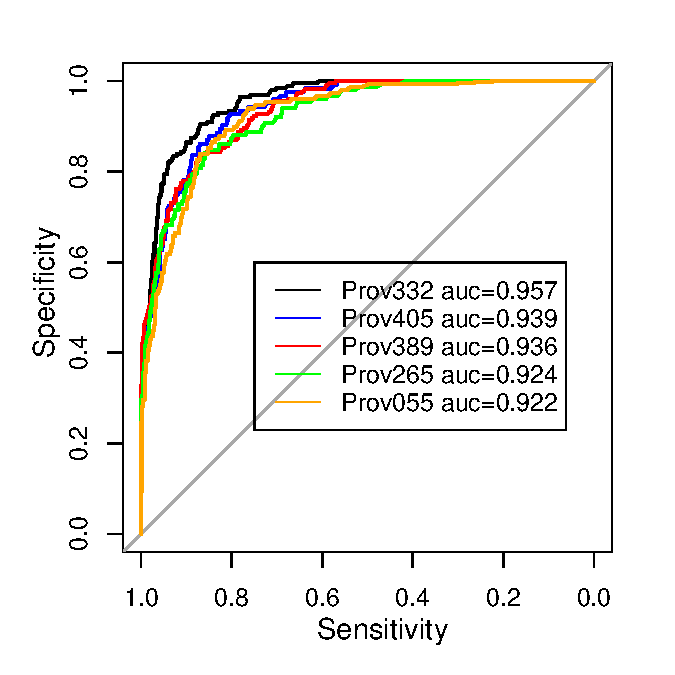
\includegraphics[width = 0.42\textwidth]{fig2/auc-top5}
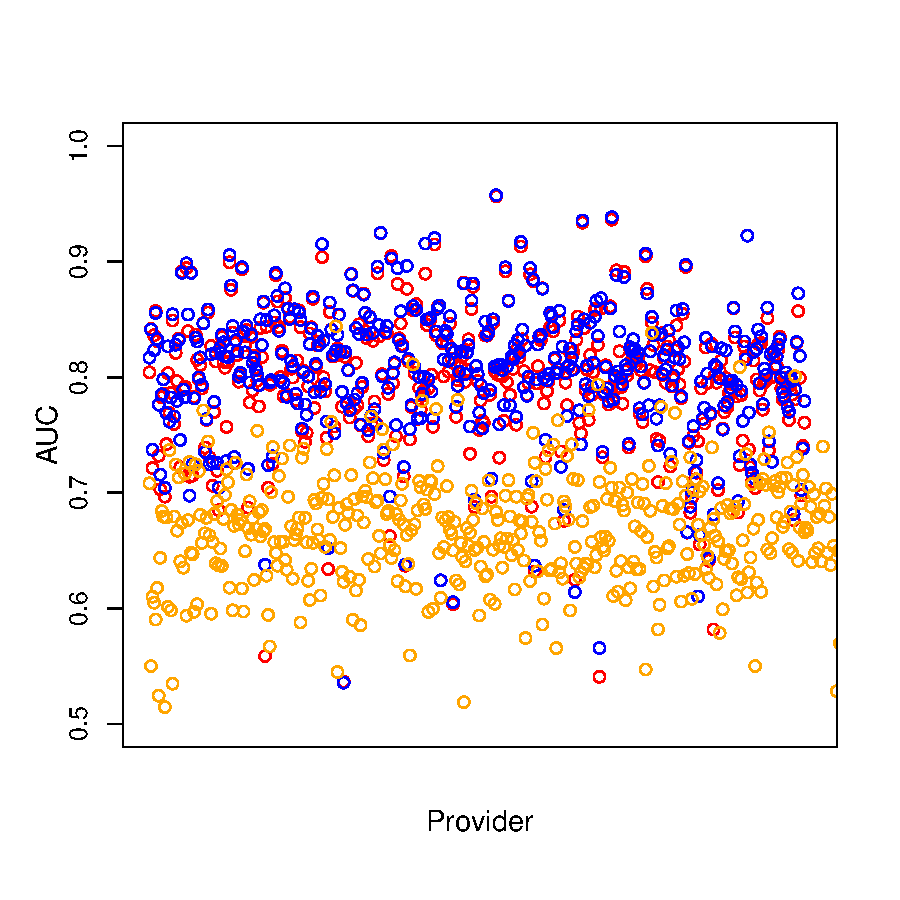
\includegraphics[width = 0.45\textwidth]{fig2/vb-by-logis-auc-sq}
\caption{ROC curves for five providers with highest AUC values using ARD predictions (left), and AUC values for provider level prediction performance comparison of Bayesian Lasso (blue), ARD (red) and basic logistic regression (orange).} \label{fig:AUCall}
\end{center}
\vspace{-1cm}
\end{figure}

In the case of ARD, we specified $a_0=1$ and $b_0=1$ for the Gamma prior of the precision parameters. In this particular application, the results are robust to the choice of hyperparameters for the models due to the fairly large amount of patient records available for each provider. Figure \ref{fig:AUCall} displays operating characteristic curves associated with the predictions on the test sets based on ARD for the five providers with the highest AUC values (left), and the AUC values for all providers using both the Lasso (blue) and ARD (red) priors. We observe that both approaches render similar prediction performance with the Lasso method performing just slightly better overall. Both models provide a similar fair to good prediction performance with an AUC $> 0.7$ for the majority of providers. The posterior mean values obtained for the penalty parameter $\lambda$ of the Bayesian Lasso vary between 0.182 and 20.3 approximately among providers. 

\begin{figure}[H]
\begin{center}
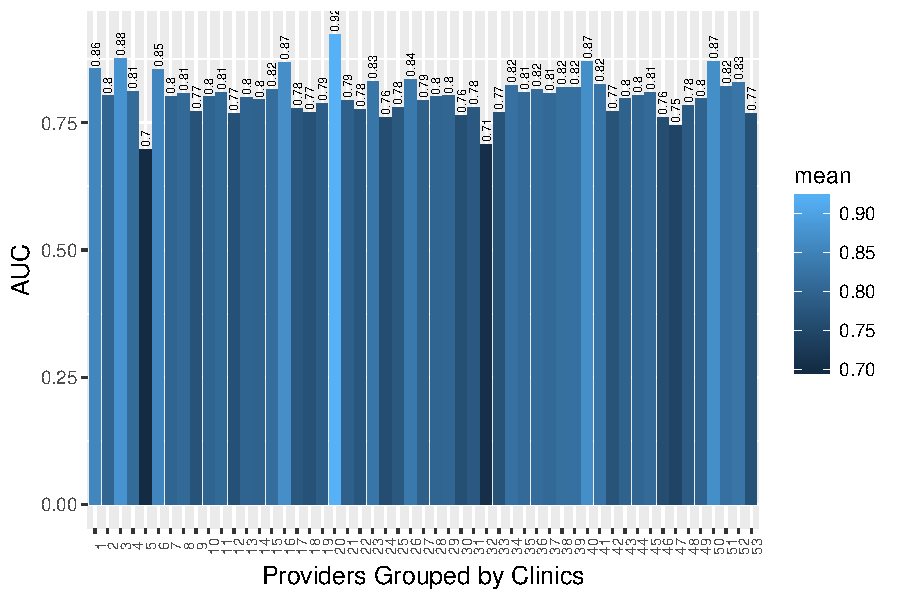
\includegraphics[width = 0.52\textwidth]{fig2/auc-grouped-by-cl4}
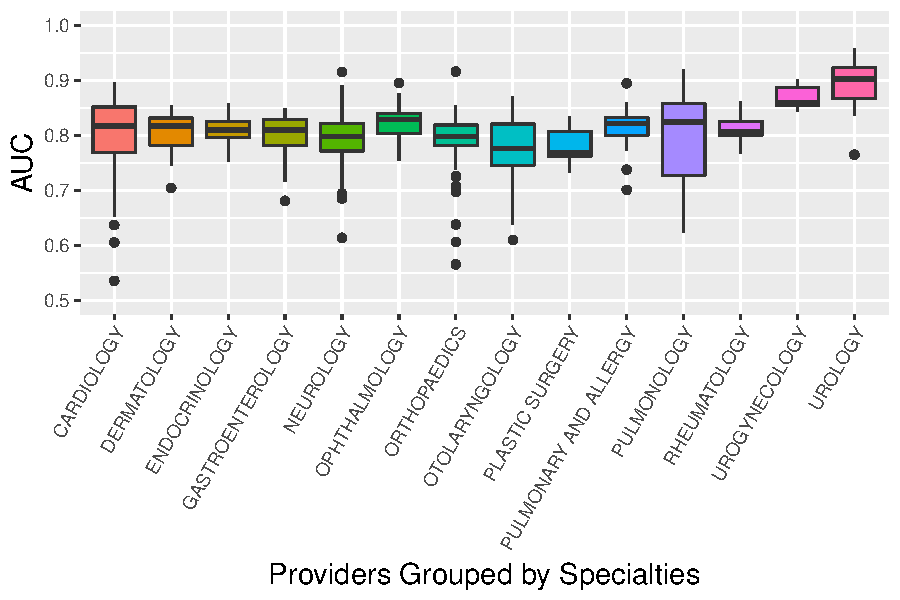
\includegraphics[width = 0.47\textwidth]{fig2/auc-grouped-by-sp-box-fixed}
\caption{Mean AUC of providers grouped into clinics (left), and box plots of AUC values for providers grouped by specialty for Bayesian Lasso method.} \label{fig:AUCgroup}
\end{center}
\end{figure}

\vspace{-0.6cm}

We also grouped the providers by clinics and specialties to explore differences in prediction performance among them. From Figure \ref{fig:AUCgroup}, we see that the average AUC among providers grouped by clinics is between 70\% and 92\%. We also observe that the prediction performance varies among providers in different specialties. For example, the highest median AUC values are observed in the Urology and Urogynecology specialties with relatively low variability among providers, while the Cardiology, Otolaringology, and Pulmonology specialties display high variability as well as the highest proportion of providers with poor prediction performance with AUC values below 0.7. We observed that the poor prediction performance for some of the providers is mostly due to relatively small training ($< 2,000$) and testing sample sizes ($< 500$).

In terms of identifying the relevant predictors of no-shows, both Lasso and ARD produce identical results. The average number of relevant features among providers is approximately 13 with a maximum of 34 predictors. We see that the relevant predictors vary significantly among providers (and specialties) such that each of the 102 covariates is relevant for at least one of the providers. Table \ref{tb:highall} displays a list of ten selected predictors whose regression coefficients are positive and therefore considered as indicators of a higher risk of no-shows. The predictors in Table \ref{tb:highall} are displayed in decreasing order according to the proportion of providers for which the specific predictor coefficient was relevant (i.e. different from zero) using the ARD estimates. From these results we observe that some predictors are fairly consistent among providers. For example, if an appointment was rescheduled or the number of days between the scheduling and the appointment date is too large the patient was more likely to be a no-show. Furthermore, patients that pay their own medical expenses (Self Pay), African American patients, patients with history of not showing to appointments in the last three months, and patients that indicated they wanted to cancel or did not confirm the appointment via the automated phone system were also more likely to not show for at least 15\% of providers. We also see that when a collection agency needs to be involved due to past unpaid bills of a patient, the relative risk of no-show increases for 46\% of providers approximately.

\vspace{-0.4cm}

\begin{table}[H]
\footnotesize
\centering
\caption{Ten most frequent relevant predictors across all providers indicating increased risk of no-show in patients.} \label{tb:highall}
\begin{tabular}{llc}
  \hline \hline
 & \bf{Predictor} & \bf{Relevance} \% \\ 
  \hline \hline
1 & Rescheduled appointment & 97.1 \\ 
2 & Days until appointment & 82.7 \\
3 & Self Pay patient (financial class)& 64.5 \\ 
4 & African American patient & 52.9 \\ 
5 & Collection agency involved & 46.4 \\ 
6 & No-show appointments in past 3 months & 22.6 \\ 
7 & Number of times appointment changed & 21.6 \\ 
8 & NC Medicaid patient (financial class)& 19.1 \\ 
9 & Wants to cancel (phone reminder status) & 16.8 \\ 
10 & Answered but not confirmed (phone reminder status) & 15.8 \\ 
   \hline
\end{tabular}
\end{table}

\vspace{-0.6cm}

\begin{table}[h]
\footnotesize
\caption{Five most frequent relevant predictors across all providers indicating lower risk of no-show in patients.}  \label{tb:lowall}
\centering
\begin{tabular}{llc}
  \hline \hline
 & \bf{Predictor} & \bf{Relevance \%} \\ 
  \hline \hline
 1 & Confirmed  appointment (phone reminder status) & 81.7 \\ 
 2 & Active in MyChart & 72.2\\ 
 3 & Age on appointment date & 55.4 \\ 
 4 & Copay due & 47.3 \\ 
 5 & Retired (employment status) & 17.2 \\  
% 6 & PREV\_APPTS\_SPEC\_24MOS & 15.6 \\ 
% 7 & PREV\_APPTS\_ALLOP\_3MOS & 15.2 \\ 
% 8 & OVERBOOKED\_YN & 13.7 \\ 
% 9 & PREV\_APPTS\_ALLOP\_24MOS & 12.5 \\ 
% 10& PREV\_APPTS\_SPEC\_3MOS & 11.6 \\ 
   \hline
\end{tabular}
\end{table}

Note that these results represent the more frequent relevant predictors of no-shows but not necessarily the strongest. The strongest predictors vary widely across providers; however, we see that appointment rescheduling and the Self Pay category of financial class are in the top two stronger predictors for approximately 90\% of the providers in this data set. Table \ref{tb:lowall} lists the top five predictors that characterize lower risk patients among providers i.e. predictors with negative regression coefficients. The top two predictors are the same for most of the providers, that is, patients that confirmed their appointments via the automated phone system and actively participated in the online portal (MyChart). We also see that older and retired patients have lower risk of no-show for a fair number of providers. Distinctive predictors are also observed among specialties, for example, having a copay has a strong negative prediction for at least 85\% of providers in Urology, Urogynecology and Pulmonology but not the other specialties.

\subsection{Results for Individual Providers} 

In this section, we discuss in more detail the interpretation of the strongest predictors of no-shows based on results from the Bayesian Lasso approach for a specific provider. The chosen provider has the best prediction accuracy in our data set with an AUC of 0.957, and serves in the Urology specialty.  
Figure \ref{fig:CI} displays the posterior means and 95\% credible intervals of the regression coefficients associated with all 99 predictors included for this particular provider (some factor categories were not present). The credible intervals tell us that the true value of the regression coefficient is in the respective interval with 95\% probability. Thus we used them to establish the relevant predictors by
identifying the regression coefficients for which the credible interval does not contain zero. We found 21 relevant predictors in this case.

\vspace{-0.35cm}

\begin{figure}[h]
\begin{center}
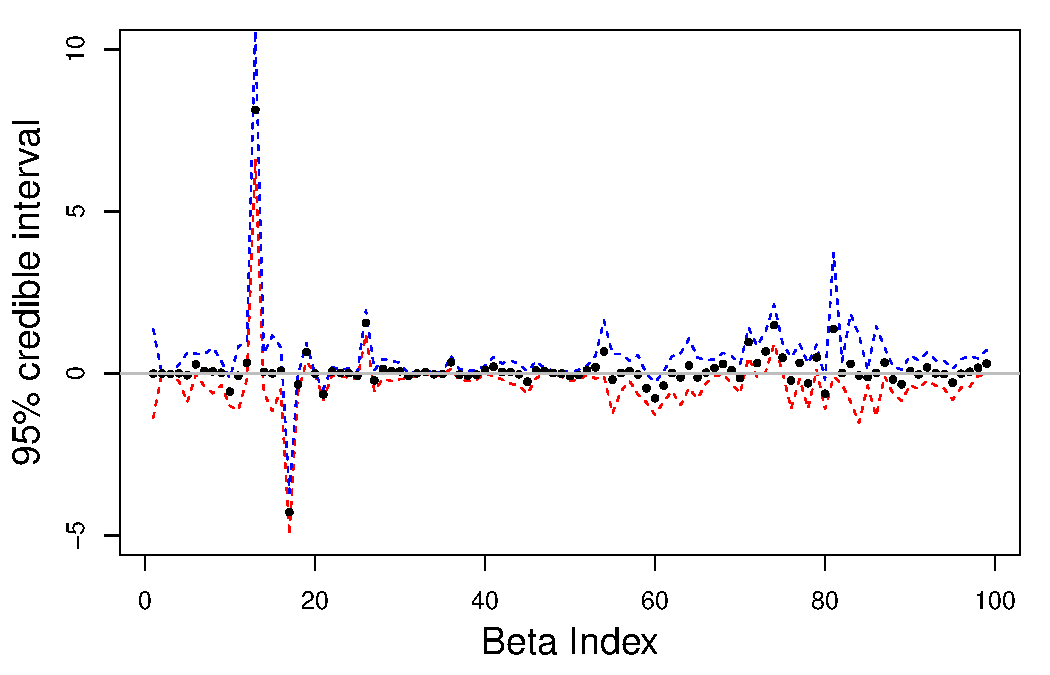
\includegraphics[width=0.55\textwidth]{fig2/Prov332-ci}
\caption{ Posterior mean estimates (dots) and 95\% credible intervals, upper limit (blue) and lower limit (red), of regression coefficients for Urology provider using Bayesian Lasso method. The horizontal line at zero is used to guide variable selection.} \label{fig:CI}
\end{center}
\end{figure}

Tables \ref{tb:highprv} and \ref{tb:lowprv} show the names and respective posterior mean and standard deviation of the coefficients for the top 14 strongest predictors, both positive and negative, in decreasing order (in absolute value). We use the estimated odds ratios (OR) to determine and compare the magnitude of the risk factors for no-shows. The odds ratio can be easily obtained by exponentiating the estimated regression coefficient associated with the predictors. Similar to what we observed in the results for all providers, the strongest no-show predictors in this case include appointment rescheduling, previous no-shows in the las three months and being in the self pay category. More specifically, holding other predictors fixed, the estimated odds that a patient with previous no-show records in the last three months does not show to the most recent scheduled appointment is 4.75 ($\hat{OR}=e^{1.56}$) greater than the corresponding odds for a patient with no history of no-shows in the last three months. Furthermore, the relative increase in the odds of no-shows is 4.44 for Self Pay patients, 2.64  for NC Blue Cross and 1.97 for Medicare Advantage patients compared to patients in the Medicare financial class (baseline category). Another strong positive predictor is past due bills that require a collection agency to be involved with an estimated odds ratio of $1.93$ ($=e^{0.66}$). Finally, the odds of no-show for a patient that answered but did not confirm the appointment through the automated phone system are 1.65 times greater than the odds of no-show for a patient that was not reached (baseline category).


\begin{table}[H]
\footnotesize
\caption{Top seven positive predictors indicating increased risk of no-show for Urology provider.} 
\label{tb:highprv}
\centering
\begin{tabular}{llcc}
  \hline   \hline
 & \bf{Predictor} & $\hat{\beta}$ & SD \\ 
  \hline  \hline
 1 & Rescheduled appointment & 8.14 & 1.05 \\ 
  2 & No-show appointments in past 3 months & 1.56 & 0.20 \\ 
  3 & Self Pay patient (financial class) & 1.49 & 0.31 \\ 
  4 & NC Blue Cross patient (financial class) & 0.97 & 0.23 \\ 
  5 & Medicare Advantage patient (financial class) & 0.68 & 0.33 \\ 
  6 & Collection agency involved & 0.66 & 0.15 \\ 
  7 & Answered but not confirmed (phone reminder status) & 0.50 & 0.20 \\ 
   \hline
\end{tabular}
\end{table}

\vspace{-0.4cm}

\begin{table}[H]
\footnotesize
\caption{Top seven negative predictors indicating lower risk of no-show for Urology provider.}
\label{tb:lowprv}
\centering
\begin{tabular}{llcc}
  \hline  \hline
 & \bf{Predictor} & $\hat{\beta}$  & SD \\ 
 \hline  \hline
  1 & Copay due & -4.28 & 0.35 \\ 
  2 & Disabled (employment status) & -0.76 & 0.25 \\ 
  3 & Previous appointments in past 3 months & -0.64 & 0.08 \\ 
  4 & Confirmed (phone reminder status) & -0.62 & 0.23 \\ 
  5 & Overbooked appotinment & -0.56 & 0.22 \\ 
  6 & Retired (employment status)  & -0.46 & 0.22 \\ 
  7 & Active in MyChart  & -0.34 & 0.14 \\ 
   \hline
\end{tabular}
\end{table}

On the other hand, for patients who have a copay the estimated odds of no-show decreases by roughly a factor of 70 for this particular provider in the Urology specialty. Demographically, patients who are disabled or retired have decreased odds of no-shows, 0.47 and 0.63 odds reduction respectively, compared to patients with an unknown employment status. Other lower risk factors for no-show patients include having previous appointments in the specific specialty in the last three months ($\hat{OR}=0.53$), confirmation of the appointment via the automated phone system ($\hat{OR}=0.54$), and being active in the MyChart online portal ($\hat{OR}=0.71$). For this individual provider we also see that the relative reduction in the odds of no-show for a patient with an overbooked appointment is 0.57 approximately.


\section{Discussion} 

We presented simple risk prediction models for no-shows that can be applied to EHR data from large health medical systems with multi-provider clinics and specialties. We discussed two Bayesian methods for adaptive shrinkage that induce sparsity in the model coefficients and allow us to identify relevant no-show risk factors. This information can be used for no-show detection and development of general intervention strategies, or to optimize booking arrangements for individual providers. Maintaining and updating multiple risk models with more incoming data can be challenging. Even though we train separate models at the provider level, models at the clinic level can also be implemented to borrow strength among providers, facilitate model maintenance and deployment, and possibly gain prediction accuracy as discussed in \cite{Ben18}.  

For big and high-dimensional data, a full Bayesian implementation of penalized regression models can be challenging and computationally restrictive. However, the use of variational approaches present an efficient alternative for model implementation within a Bayesian framework with relatively low accuracy loss. Other Bayesian methods based on spike-and-slab priors \citep{GeorgeMcCulloch93} provide a more principled approach to variable selection. In contrast to penalized regression, this approach includes natural measures of uncertainty such as posterior inclusion probabilities of the individual predictors and formal model selection using Bayes factors. We refer the reader and practitioners to the work of \cite{carbonetto
17}  and the \texttt{varbvs} package in R which implements the spike-and-slab prior for Bayesian variable selection in large-scale regression based on variational approximation methods. 

Penalized regression approaches such as the ones presented in this paper can be vastly adapted to hospital scheduling systems. By inputting the basic information of a patient the models can accurately predict a person's probability of not showing to a scheduled appointment. Preventive measures can then be taken to reduce no-show rates such as increasing the number of reminder calls or scheduling in more patients depending on this days' patient probability of being a no-show,  similar to the overbooking scheme used by airline companies. However, intervention strategies should be planned with care to avoid the implications of a model that effectively discriminates against certain subpopulations. The work of \cite{Kusner17} introduces the concept of \emph{counterfactual fairness} to enforce that the distribution over possible predictions for an individual should remain unchanged when an individual's protected attributes, as is the case of race and socioeconomic status, had been different in a causal sense. This approach could be explored in future work to overcome discrimination patterns in the decision-making process since simply removing the protected attributes from the analysis is not a satisfactory solution.

\bibliography{references}

\appendix
\section*{Appendix A.}

Using the fact that the Laplace prior can be expressed as a scale mixture
of normals with exponential mixing density \citep{ParkCasella08}, the hierarchical representation of the Bayesian Lasso model is the following:
\begin{align*}
\beta & \sim N(0,D)\\
D &= diag(d_1,d_2,...,d_p)\\
d_1, d_2, \ldots, d_p & \stackrel{iid}{\sim} \exp(\lambda^2/2)\\
\lambda^2 & \sim \Gam(r,\delta).
\end{align*}
The binomial likelihood can also be represented as a mixture of
normals with Polya-Gamma mixing distribution using the latent variable data augmentation approach of \cite{PolsonScott13}. A Polya-Gamma Distribution is $w \sim \PG(a,c)$ with density function given by
\begin{equation*}
p(w|a,c)=\frac{exp(-\frac{c^2}{2}w)p(w|a,0)}{\mathbf{E}(exp(-\frac{c^2}{2}w))}.
\end{equation*}

Given the conjugate hierarchical representation of the model for Lasso penalized logistic regression, the full conditionals for Gibbs sampling are given in closed form as follows:
\begin{align*}
w_i | x_i, \bbeta & \sim \PG(1,x_i\bbeta) \\
\bbeta | \lambda, d_{1:p}, y_{1:n}, w_{1:n} & \sim N_p(m_n,V_n)\\
1/d_{1:p} | \bbeta, \lambda & \sim \IGau \left(\sqrt{\frac{\lambda^2}{\beta_j^2}},\lambda^2 \right)\\
\lambda^2| d_{1:p}  & \sim \Gam \left( r + p, \delta + \sum_{j=1}^p d_j/2 \right)
\end{align*}
where $\IGau$ represents the Inverse Gaussian distribution, and
\begin{align*}
V_n & = (D^{-1} + X^T\Omega X)^{-1}\\
m_n & = V_n X^T\boldsymbol{k}
\end{align*}
for $\Omega  = diag(w_1, w_2, \ldots, w_n)$ and $\boldsymbol{k} = (k_1, k_2, \ldots, k_n)$ where $k_i = y_i - 1/2$.
\end{document}


